\documentclass{acm_proc_article-sp}


\usepackage{graphicx}
\usepackage[lined,boxed,commentsnumbered]{algorithm2e}
\usepackage[normalem]{ulem}
%\usepackage{algorithm2e}
%\usepackage{draftwatermark}
% path to spreadsheet with test data and graphs: "Google Drive\Doutorado\Pesquisa\Testes\WsnEE\"
% file name: "WsneeFD - Experimental Data + Grafs - 1000 Cycles - Averages (Fernando) - 19082014.ods"
% sub-path to graphic files: "Gráficos\Gráficos BCWSN SD=1 CD=5"
% path to files for upload project: "Google Drive\Doutorado\Pesquisa\Artigos\SAC2015\SACLatex"


% correct bad hyphenation here
\hyphenation{op-tical net-works semi-conduc-tor sche-dul-ing}
\newcommand{\dia}{\hspace*{.1cm} \hfill $\diamond$}


\begin{document}
%

\title{Using Fractal Clustering to explore Behavioral Correlation: A new
approach to reduce energy consumption in WSN}

% author names and affiliations
% use a multiple column layout for up to three different
% affiliations
% \author{\IEEEauthorblockN{Fernando Rodrigues}
% \IEEEauthorblockA{University of Fortaleza\\Fortaleza - Ceara - Brazil\\
% fernandorodrigues@edu.unifor.br}
% \and
% \IEEEauthorblockN{Angelo Brayner}
% \IEEEauthorblockA{University of Fortaleza\\
% Fortaleza - Ceara - Brazil\\
% brayner@unifor.br}
% \and
% \IEEEauthorblockN{Jose E. Bessa Maia}
% \IEEEauthorblockA{State University of Ceara\\
% Fortaleza - Ceara - Brazil\\
% jose.maia@uece.br}}


% make the title area
\maketitle


\begin{abstract}

Sensor clustering is an efficient strategy to reduce the number of messages
flowing in a Wireless Sensor Network (WSN).
This paper presents a new approach to cluster sensors in WSNs, called
Behavioral Correlation in WSN (BCWSN), which is based on the behavior of recent
historical data collected by sensors. Instead of using spatial distance among
sensors, the proposed approach uses the concepts of difference in magnitude and
trend of sensed data. For clusters maintenance, BCWSN implements the notion of
Fractal Dimension to dynamically find the best configuration for clusters. In
order to validate our approach, simulations have been conducted over real data.
The results show that, with 5\% error threshold in temporal correlation, BCWSN
can reduce the number of messages injected into the network up to 94.80\% over a
naive approach (no clustering, no prediction and no suppression) and up tp
57.24\% when compared to approaches implementing temporal correlation, while
RMSE remains roughly stable.

\end{abstract}

\category{H.2.m}{Database Management}{Miscellaneous}

\terms{Algorithms, Measurement, Performance}

% keywords
\keywords{Wireless sensor networks, Behavioral Correlation, Fractal clustering}




\section{Introduction}
% no \IEEEPARstart

Advances in wireless communication have enabled the development of massive-scale
wireless sensor networks (WSNs). Sensors nodes are devices used to measure
physical phenomena from the environment. They are limited in power,
computational capacity, and memory. In a WSN, sensors are usually scattered in
the network and use low-power communication channels to disseminate collected
data to a base station, from which the information (query) was originally
requested. Due to these characteristics, WSNs have been widely used for
environmental monitoring (e.g., traffic, habitat), industrial sensing and
diagnostics (e.g., factory, supply chains), infrastructure protection (e.g.,
water distribution), battlefield awareness (e.g., multi-target tracking) and
context-aware computing (e.g., intelligent home) applications
\cite{MaiaSAC2013}.
\vspace*{-.3cm}

In spite of advances in WSN technology, a critical key point is still energy
consumption of sensor nodes. As a matter of fact, communication among sensors is
by far the activity which consumes more energy in a WSN. By reducing
communication costs, energy power may be drastically saved, consequently
increasing WSN's lifetime. An effective strategy to reduce energy consumption
is, therefore, to reduce the number of messages sent across the network.
Nevertheless, the less the number of sensed data is transmitted, the lower the
accuracy of results provided by a WSN. Thus, higher accuracy in WSNs comes at a
higher energy cost.
\vspace*{-.3cm}

Clustering sensor nodes in a WSN may reduce the number of messages flowing in a
WSN. This is because the Cluster Heads, which are responsible for a set of
sensor nodes, coordinate the data flow (messaging) between sensors and the sink.
By doing that, the Cluster Head (CH) forward to the sink node "important"
messages. Several approaches have been implemented to form clusters in WSNs,
where most of them are based on spatial correlation of the sensors of the WSN.
\vspace*{-.3cm}

So far, it is well known that data collected by WSNs is spatially or temporally
correlated \cite{Chu2006, Villas2012, Yoon2005}. Temporal correlation states
that it is very likely that readings sensed in a lapse of time by a given node
have very nearly values (temporal locality). This property makes possible to
predict (with a given error threshold) future sensed values based on data
collected in the past. On the other hand, spatial data correlation is related to
the idea that physical proximity among sensors may lead to similar measurements
(values) of sensed data (spatial locality). Thus, it is possible to estimate
values sensed by sensors in a region R based on the readings of a sensor S
located in R as well.
\vspace*{-.3cm}

However, in several scenarios, sensors which are not spatially close to each
other may also have similar data reading patterns. In order to illustrate this
statement, consider a dense WSN deployed to monitor forest fires.
Now, suppose a scenario in which the monitored region is affected by dozens of
small forest fires. Figure \ref{fig:contour_lines} depicts possible temperature
contour lines for this situation. Observe in Figure \ref{fig:contour_lines} that
there are several closed regions, which represents fields with forest fire area.
The temperature measurements sensed by sensors in those spatially separated
regions present high correlation. In such cases, traditional spatial data
correlation techniques, using physical distance among sensors, are not efficient
to detect spatial correlation. Consequently, it is not adequate for being
applied as a criterion to cluster sensors in a WSN.

\begin{figure}[!htb]
\centering
	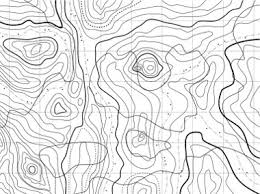
\includegraphics[scale=0.8]{I2.png}
    \caption{Contours lines of temperature}
    \label{fig:contour_lines}
\end{figure}
\vspace*{-.3cm}


For that reason, we propose a new approach for detecting data correlation among
data produced by a WSN. The main goal of the proposed approach, called  {\it
Behavioral Correlation}, is to identify similar patterns of sensor readings
even in sensors geographically distant from each other. Behavioral Correlation
is computed from the time series of sensor readings by applying {\it
Similarity Measure} \cite{Liu2007}. This way, Behavioral Correlation is able to
capture difference in magnitude and trend of sensed data instead of using
spatial distance among sensors for identifying spatial correlation among data.
\vspace*{-.3cm}

Based on the concept of Behavioral Correlation, this paper presents a new
approach for clustering sensors in WSNs, called Behavioral Correlation in WSN
(BCWSN). The idea is to apply Behavioral Correlation for defining an initial
cluster configuration in a WSN.
\vspace*{-.3cm}

Behavioral Correlation may vary in time, which can in turn impose modification
on the initial cluster configuration. Thus, for clusters maintenance, BCWSN
implements the notion of Fractal Dimension to dynamically find the best
configuration for clusters. The idea is to apply fractal dimension to verify if
the Behavioral Correlation computed for defining the initial cluster
configuration is still valid. This method is triggered whenever new data arrives
at the sink.
The sink will analyze, through the Minimum Difference of Fractal Dimension,
whether such data are just "noise" or actually they represent "novelties". 
Nevertheless, in order to avoid that every sensed data be transmitted to the
sink node, a regression model is applied to compute data temporal correlation.
\vspace*{-.3cm}

The remainder of this document is organized as follows: Section
\ref{related-work} describes related work and outlines the differences between
our method and existing methods. In Section \ref{implementing-bcwsn}, the
proposed Behavioral Correlation in WSN (BCWSN) method and the sensor-scheduling
policy are presented and discussed. Simulations with a Sinalgo
\cite{Sinalgo2007} prototype executed over real sensor data are presented and
discussed in Section \ref{eval}. Finally, Section \ref{conclusion} concludes the
paper.


\section{Related Work}
\label{related-work}

In EEDC \cite{Liu2007}, measures of dissimilarity are calculated by the sink
node for pairs of nodes based on up to $3$ parameters, namely: {\it (i)}
differences in magnitude (\textit{M}) and {\it (ii)} trend (\textit{T}) of the
data values and {\it (iii)} geographical/euclidean distance between nodes
($g_{max}dist$).
The criterion of formation of clusters is based on the maximum threshold of
dissimilarity (max\_dst) defined by a tuple (\textit{M}, \textit{T},
$g_{max}dist$). It works as follows: $1)$ Initially, the sensed data by each
node are sent in the form of a temporal series for the sink. $2)$ Then the sink
stores all the data from the sensors and afterwards calculates the measure of
dissimilarity for each pair of nodes of the network. $3)$
With the calculated measures and the maximum threshold of dissimilarity
(max\_dst), the sink divides the nodes into clusters.
That work does not take into account the energy reserve of each node as a
criterion for choosing representative nodes (it is used an algorithm that makes,
simultaneously, the equitable scheduling - round robin - along with the random
choice of representative nodes). In this work, we chose Cluster Heads according
to the remaining energy level and the minimum distance to the sink. Moreover,
unlike \cite{Liu2007}, we can take into account readings from multiple different
data types by sensors.
\vspace*{-.3cm}

Carvalho \textit{et al.} \cite{Carvalho2011} proposed applying Multivariate
Spatio-Temporal Correlation to improving prediction accuracy in a WSN. However,
that work does not reduce the energy consumption of the network. In fact, it
even increases the energy consumption of the network in many situations. In our
work, using multiple linear regression with Fractal Clustering, we achieved the
reduction of the overall energy consumption of the network, obtaining results
with a Root Mean Square Error (RMSE) for the prediction data (w.r.t. the sensed
data) even smaller than other approaches.
\vspace*{-.3cm}

Barbar\'{a} and Chen \cite{Barbara2000} proposed a method, called {\it Fractal
Clustering} (FC), to cluster datasets. In that work, an initialization step
based on the nearest neighbor strategy creates the initial clusters. Then, it
implements the algorithm of incremental step, which uses \textit{Fractal
Dimension} calculation based on an implementation of Box Counting algorithm,
called FD3 \cite{Liebovitch1989}. In our work, an extended version of FC
method is proposed (BCWSN). In our case, sink uses Similarity
Measure (see Step 2 in Section \ref{implementing-bcwsn}) in the initialization
step to form initial clusters. \sout{An in-network data prediction strategy is used in
order to avoid that every sensed data be transmitted to the sink node.} However,
Behavioral Correlation \sout{environmental conditions} may vary in time at some sensed regions. For that
reason, new data can arrive at the sink. Thus, we implemented a ``special''
Fractal Clustering algorithm (see Step 5 in Section \ref{implementing-bcwsn})
for clusters maintenance, which avoids a bulk of messages to receive the data
reading of all sensors from the same involved clusters, since FC needs only
``real'' new data.

\section{Implementing Behavioral Correlation in WSNs}
\label{implementing-bcwsn}

In order to build an initial cluster configuration, BCWSN implements the idea of
Similarity Measure, which is responsible for computing Behavioral Correlation.
Behavioral Correlation may vary in time, which can in turn impose modification
on the initial cluster configuration. For that reason, BCWSN implements the
concept of fractal dimension. In our proposal, a sensor network consists of a
sink node (a.k.a. base station or fusion center) and a set of sensor nodes
scattered in a region.
Thus, whenever new data arrive at the sink, it analyzes them, through the
Minimum Difference of Fractal Dimension method (described below) for identifying
if such data are just ``noise'' or ``novelties''. If the value of Minimum
Difference of Fractal Dimension (MDFD) is above a certain threshold, or if a
maximum number of noise for a given sensor node is reached, then it will
trigger the process of splitting cluster.
Otherwise, the sensor node (that sent the ``novelties'') will be relocated to
the chosen cluster, i.e., one that has a smaller difference in Fractal Dimension
with the inclusion of new data.
\vspace*{-.3cm}



%\subsection{The BCWSN Mechanism}
BCWSN can be divided into five steps as described next.
\vspace*{-.3cm}

%\subsubsection{Learning Stage}
{\bf Step 1 - Learning Stage}
In this step, the sink node collects sensed data from all sensors belonging to
the network in order to compute the initial cluster formation and the
coefficients of the linear regression equation (see Step 3). Thus, the sink 
node firstly sends a broadcast message to all
nodes of the network, requesting the following data from sensors:
battery level, spatial location and sensed values. The amount of data used by the
learning stage is a parameter, denoted \textit{initial slot time}, which should be
defined by the application expert (e.g. 70). Each sensor answers the broadcast
message from sink in a batch mode, i.e., it makes all sensing tasks required and
sends only one message response to sink node with all reading data.
\vspace*{-.3cm}

%\subsubsection{Clustering Sensor Nodes}
{\bf Step 2 - Clustering Sensor Nodes}
%\label{clustering-sensors}
As mentioned before, the BCWSN mechanism clusters sensor nodes by means of
Behavioral Correlation. A \textit{similarity measure} (based on \cite{Liu2007})
is used in order to compute Behavioral Correlation. Thus, sensors with similar
data reading pattern for all sensed data type are grouped into a single cluster.
The similarity measure among sensed data of two different sensors is defined by
similarity of magnitude and similarity of trend, as described next.
\vspace*{-.3cm}

\newtheorem{defini}{Definition}

\begin{defini}
Similarity of magnitude-M: Two sensors ($S$ and $S'$) with time series
$S$=\{$s_{1}$,$s_{2}$,\ldots,$s_{n}$\} and
$S'$ = \{$s'_{1}$,$s'_{2}$,\ldots,$s'_{n}$\} are magnitude-M similar if 
\begin{equation}
\label{equ:magni}
\frac{\sum_{i=1}^{n} |s_{i}-s'_{i}|}{n} \leq M
\end{equation}
\dia
\end{defini}
\vspace*{-.9cm}

\begin{defini}
Similarity of trend-T: Two sensors ($S$ and $S'$) with time series
$S$=\{$s_{1}$,$s_{2}$,\ldots,$s_{n}$\} and
$S'$=\{$s'_{1}$,$s'_{2}$,\ldots,$s'_{n}$\} are trend-T similar if 
\begin{equation}
\label{equ:trend}
\frac{P}{n} \geq T,
\end{equation}
where $n$ is the total number of sensed data and $P$ is the number of pairs
$(s_{i},s'_{i})$ in the time series which satisfy $\nabla s_{i} \times \nabla
s'_{i} \geq 0$, where $\nabla s_{i} = s_{i} - s_{i-1}$, $\nabla
s'_{i} = s'_{i} - s'_{i-1}$ and $1 < i \leq n$.
\dia
\end{defini}
\vspace*{-.5cm}

Thus, sensors which are magnitude-M and trend-T similar for all sensed data type
are grouped in the same cluster (M and T defined by the application expert).
After all time series of all sensors in a WSN have been processed during the
learning phase, the initial WSN cluster configuration is defined by the sink.
\vspace*{-.3cm}

Once the sensors are initially grouped into clusters, the Cluster Head of each
cluster is defined by applying the energy level criterion.
In other words, for each cluster, the Cluster Head is the node with the highest
energy level. In the case of nodes with same energy level, the node with the
shortest distance to the sink node is chosen.
\vspace*{-.3cm}

%\subsubsection{In-Network Data Prediction}
{\bf Step 3 - In-Network Data Prediction}
%\label{data-predict}
The in-network prediction implemented by BCWSN relies on the
following linear regression equation, applied for each sensed data type:
$\hat{S}(t) = a + bt$.
The time $t$ is an independent variable. $\hat{S}(t)$ represents the estimated
value of $S(t)$ and it is variable with $t$. Parameter $a$ is the interceptor-t
(value of $\hat{S}(t)$ for $t=0$) and $b$ is the stretch slope, and are computed
as follows:
\begin{equation}
\label{coef-a}
	a = \frac{1}{N}\left(\sum S_{i} - b\sum t_{i} \right) = \bar{S} - b\bar{t},
\end{equation}
\vspace*{-.3cm}
\begin{equation}
\label{coef-b}
	b = \frac{\sum \left(t_{i} - \bar{t}\right)\left(S_{i} - \bar{S}\right)}{\sum \left(t_{i} - \bar{t}\right)^{2}}.
\end{equation}
	\dia
\vspace*{-.4cm}

The idea behind this method is that both the sink and the sensor node know the
regression equations to predict the sensed values for all sensed data. Thus, a
sensor node does not need to send any data to sink, since it is able to predict
all sensed data by the sensors. Then, the network is saving power of sensors
\cite{MaiaACR2013}.
\vspace*{-.3cm}

During the Learning Stage, the sink node computes the initial coefficients $a$
and $b$ for each sensed data type, for each sensor node, based on the time
series received from them. Thereafter, the sink node sends the calculated
coefficients to the respective sensors.
\vspace*{-.3cm}

%\subsubsection{Sensing}
{\bf Step 4 - Sensing}
As mentioned before, one sensor node (Cluster Head) in each cluster $C_{i}$ is
selected to coordinate the data sensing activity carried out by all nodes in
$C_{i}$.
\vspace*{-.3cm}

After a node receives the corresponding coefficients, it starts using these
coefficients in reading / prediction loop.
Whenever a sensor node senses values \{$v_{1}$,$v_{2}$, \ldots,$v_{n}$\} of
certain data type \{$d_{1}$,$d_{2}$,\ldots,$d_{n}$\}, it verifies if anyone of
$v_{n}$ is not within a ``tolerable difference'' $t$, i.e., $v_{n} \not \in
[p_{n}-t,p_{n}+t], t \geq 0$, let $p_{n}$ be the predicted value by applying
the regression equation corresponding to data type $d_{n}$. Any data outside the
tolerable difference are treated as ``novelty'' for the model.
``Tolerable difference'' is a parameter, set by the application expert (e.g.
$5\%$ or $10\%$).
\vspace*{-.3cm}

Whenever a sensor node $s$ detects a given amount of novelties $n$ (or ``Sensor
Delay'', defined by the application expert), it sends the novelties as a
notification to the Cluster Head of the cluster to which $s$ belongs. 
Cluster Head in turn logs the number of notifications, in such a way that when
the number of received notifications is greater than a preset limit $m$ (or
``Cluster Delay'', also defined by the application expert), the CH sends a
message to the sink for computing new regression coefficients for that cluster.
\vspace*{-.3cm}

%\subsubsection{Fractal Clustering}
{\bf Step 5 - Fractal Clustering}
%\label{cluster-maintenance}
In the proposed approach, the sink has the ability to automatically and
autonomously maintain the clusters. The strategy is to maintain the sensor
clusters according to the Minimum Difference of Fractal Dimension (MDFD).
\vspace*{-.3cm}

Considering the Fractal Clustering (Algorithm \ref{alg:MDFD}), let $R_{new}$ be
the new reading data to be treated by the sink; let $S_{R}$ be the sensor which
report that ``novelties'' (i.e. new reading - $R_{new}$) to the sink node; let
$C_i$ be the $i-th$ sensor cluster, formed by a CH and other cluster members (0
or more sensors); let $D(C_i)$ be the data (sensor's data) of cluster $C_i$; let
$D'(C_i)$ denote the data of cluster $C_i$ with the new reading data $R_{new}$
(i.e. $D'(C_i) = D(C_i) \cup R_{new}$) and let $F_{d}(D(C_i))$ be the value of
Fractal Dimension of the data of cluster $C_i$.
\vspace*{-.6cm}

In the phase of sensor node clustering (Step 2), the Fractal Dimension is 
calculated and stored for each initial cluster
($F_{d}(D(C_i)), \forall i$). The idea is to find out which cluster
$C_{\hat{\imath}}$ the inclusion of new sensor data $R_{new}$ will take to produce
the slightest change in its Fractal Dimension.
\vspace*{-.3cm}

MDFD strategy is as follows:
whenever the sink receives "novelties", i.e. new data ($R_{new}$), from a CH on
a given cluster $C_j$, it calculates which cluster $C_i$ has the minimal
\textit{fractal impact} with the addition of new data, i.e. the minimum absolute
difference between the previous Fractal Dimension value (calculated before the
new data arrives) ($F_d(D(C_i))$) and the new one ($F_d(D'(C_i))$), where:
$D'(C_i) = D(C_i) \cup R_{new}, \forall i$.
\vspace*{-.3cm}

Let {\it min}$\nabla$ be the minimal difference ($|F_d(D'(C_{\hat{\imath}})) -
F_d(D(C_{\hat{\imath}}))|$, where $\hat{\imath} = min(|F_d(D'(C_i)) - F_d(D(C_i))|),
\forall i$). If {\it min}$\nabla$ is greater than a certain threshold ($\tau$) -
defined by the application expert (e.g. $\tau = 0.03$), then this new data
$R_{new}$ will simply be rejected as noise and a sequential noise counter
(NoiseCount) is incremented for the current sensor.
\vspace*{-.3cm}

Otherwise, if {\it min}$\nabla$ is greater than a split threshold ($\sigma$)
(e.g. $\sigma = 0.1$) or if the NoiseCount is greater than a maximum number of
sequential noise ($\mu$) (defined by the application expert - e.g. $\mu$ = 3),
then a split process is triggered.
\vspace*{-.3cm}

On the other hand, if the chosen cluster $C_i$ is the same $C_j$ (i.e.
$i=j$), the sink will just calculate new coefficients ($a$ and $b$, equations
(\ref{coef-a}) and (\ref{coef-b})) to the corresponding sensor in this cluster.
Otherwise, the sink must remove this sensor node ($S_{R}$ with new data
$R_{new}$) from its old cluster $C_j$ and add it to the new cluster $(C_i)$.
The Algorithm \ref{alg:MDFD} outlines this strategy.
%\vspace*{-.3cm}

\begin{algorithm}
 \SetAlgoLined
 \LinesNumbered
 \small
 \KwData{input parameters: set of all K current sensor clusters (\{$C_i \vert 1
 \leq i \leq K$\}), values of Fractal Dimension of all current sensor clusters
 ($F_d(D(C_i))$), sensor node($S_{R}$) with new data ($R_{new}$), noise
 threshold ($\tau$), split threshold ($\sigma$), maximum sequential noise
 ($\mu$)}
 \KwResult{processes Fractal Clustering}
 Sink Node receives new data ($R_{new}$) from sensor ($S_{R}$) of cluster $C_j$\;
 \For{i = 1 \ldots K}{
	  Compute $F_d(D(C_i))$\;
	  Let $D'(C_i) = D(C_i) \cup R_{new}$\;
	  Compute $F_d(D'(C_i))$\;
 }
  Find $\hat{\imath} = min(|F_d(D'(C_i)) - F_d(D(C_i))|)$\;
  \uIf{$|F_d(D'(C_{\hat{\imath}})) - F_d(D(C_{\hat{\imath}}))| > \sigma$ OR numSeqNoise > $\mu$}{
  	SplitCluster($C_j$)\;
  } 
  \uElseIf{$|F_d(D'(C_{\hat{\imath}})) - F_d(D(C_{\hat{\imath}}))| > \tau$}{
  	numSeqNoise++\;
  } 
  	\uElseIf{$j \neq \hat{\imath}$}{
  		Remove $S_{R}$ from cluster $C_j$\;
  		Place $S_{R}$ in cluster $C_{\hat{\imath}}$\;
  	}\uElse{
    	Replace $S_{R}$ in cluster $C_{\hat{\imath}}$\;
    }
 \caption{Fractal Clustering algorithm - FC strategy}
 \label{alg:MDFD}
\end{algorithm}


\section{Empirical Evaluation}
\label{eval}

In order to show the potentials of the proposed approach, simulations over real
data have been conducted and the main results achieved so far are presented and
discussed in this section. 

\subsection{Implementation}
\label{implementation}

The simulation prototype has been implemented in Java, exploiting the facilities
provided by Sinalgo \cite{Sinalgo2007}, a well-known framework for testing and
validating network algorithms. The experiments have been executed on i7 computer
with 8 GB RAM and Mac OS X as operating system.
One of the main reasons for choosing Sinalgo is because it is very scalable in
nature, allowing that experiments with up to several thousands of sensor nodes
may be executed in a reasonable time. The data used for the simulation were
extracted from the real data of experiment Intel Lab Data \cite{Intel2004}. 

\subsection{Simulation Setup}
\label{data-and-experiments}

M-magnitude parameter has been configured with the value of $1.5$ and T-trend
was $5\%$, the same as the error threshold (t). The amount of initial data sensing
(initial slot time) was 70 readings, used for the learning stage.
\vspace*{-.3cm}

The performance evaluation was done through different applications, which we used
to simulate and compare three approaches of a monitoring application. 
This monitoring application simulates the gathering of two variables from the
environment: ``temperature'' and ``humidity''.
In the experiments, we have executed the following approaches: {\it
  (i)} Naive approach \cite{Madden2005}, in which all nodes send their sensed
data to the sink node;  {\it
  (ii)} Adaga-P* approach \cite{MaiaSAC2013, MaiaACR2013}, which
implicitly implements spatial correlation to cluster sensors and exploits the
benefits of using a linear regression model to reduce the number of messages
injected into the network, and;  {\it 
  (iii)} BCWSN approach, which implements Behavioral Correlation, with the
  maintenance of clusters through \textit{FC} strategy.
\vspace*{-.3cm}

In order to compare the aforementioned approaches, two metrics have been
deployed: 1) The Root Mean Square Error (RMSE) to verify the accuracy of
approach, and; 2) The Number of Messages injected into the network, which is a
critical factor to measure energy consumption of the network. The RMSE is
calculated by reference to the naive approach filtered values.
The simulation parameters are presented in Table \ref{tab:parameters}.

\begin{table}[h!]
\tiny 
\caption{Simulation parameters}
\label{tab:parameters}
\begin{center}
\begin{tabular}{|l||l|}
\hline
Parameters &Values\\
\hline\hline
Sink node: number (position) &1 (center) \\
\hline
\# of nodes &54 \\
\hline
\# of cycles executed &1000 \\
\hline
Notification rate (per second) &31 \\
\hline
Sensed data types &Temp. / Hum. \\
\hline
Initial slot time (\# learning stage) &70 \\
\hline
M-magnitude &1.5 \\
\hline
T-trend &0.05 \\
\hline
Tolerable difference {\it(t)} &0.05 \\
\hline
Sensor delay {\it(n)} &1 \\
\hline
Cluster delay {\it(m)} &5 \\
\hline
FC noise threshold ($\tau$) &0.03 \\
\hline
FC split threshold ($\sigma$) &0.1 \\
\hline
FC maximum sequential noise ($\mu$) &3 \\
\hline
\end{tabular}
\end{center}
\end{table}
\vspace*{-.3cm}


\subsection{Results and Discussion}
\label{results-and-discussion}

Firstly, we show and analyze the results for {\it temperature}. Since in Naive
approach the RMSE is $0$, Table \ref{tab:rmse} presents the average (AVG),
standard deviation (STD), maximum (MAX) and minimum (MIN) value of RMSE only for
Adaga-P* and BCWSN.
\vspace*{-.3cm}

Looking more closely to Tables \ref{tab:rmse} and \ref{tab:num-msg}, one can
observe that BCWSN presents a RMSE with average $0.443$ and standard deviation
$0.1028$. RMSE produced by BCWSN is $6.3\%$ higher in average than RMSE
presented by Adaga-P*. Nevertheless, the average of the number of transmitted
messages in BCWSN is $94.80\%$ smaller than the Naive approach (see Table
\ref{tab:num-msg}). Compared to Adaga-P*, the average of messages exchanged in
BCWSN is $57,24\%$ lower.
\vspace*{-.3cm}

\begin{table}[h!]
\small
\caption{RMSE per round - Temperature}
\label{tab:rmse}
\begin{center}
\begin{tabular}{|l||l|l|l|l|}
\hline
RMSE &AVG &STD &MAX &MIN \\
\hline\hline
Adaga-P* &0.4168 &0.0499 &0.469 &0 \\
\hline
BCWSN &0.443 &0.1028 &1.158 &0 \\
\hline
\end{tabular}
\end{center}
\end{table}
%\vspace*{-.5cm}

It is important to observe that in Table \ref{tab:num-msg}, the values for
column MIN for Adaga-P* and BCWSN are equal to zero. This is because in several
rounds the predicted (see Section \ref{implementing-bcwsn}) value is equal to
the sensed value. In this case, the sensor does not need to forward the sensed
value. In some situations, sensor nodes from different clusters may send 
messages to the sink (through their Cluster Heads), because changes are
occurring in the sensed environment. For that reason, the Standard Deviation of
number of message in BCWSN is greater than in Adaga-P* (Table
\ref{tab:num-msg}).

\begin{table}[h!]
\small
\caption{Number of messages per round - Temperature}
\label{tab:num-msg}
\begin{center}
\begin{tabular}{|l||l|l|l|l|}
\hline
Num Msg &AVG &STD &MAX &MIN \\
\hline\hline
Naive &224 &0 &224 &224 \\
\hline
Adaga-P* &27.257 &24.8360 &198 &0 \\
\hline
BCWSN &11.654 &49.5202 &607 &0 \\
\hline
\end{tabular}
\end{center}
\end{table}
\vspace*{-.3cm}


Figure \ref{fig:rmse} depicts the evolution of RMSE per round. The RMSE in 
Adaga-P* approach tends to get very close to $0.47$ at about $1000$ cycles,
while the BCWSN stabilizes at about $0.39$ at the same moment. Thus, BCWSN
provides an efficient compromise between accuracy and reduction in energy
consumption, since it reduces the communication activity (see Table
\ref{tab:num-msg}). It is important to note that in the Naive approach the RMSE
is always 0 (zero), because all sensors send all sensed data to the sink.
\vspace*{-.3cm}

\begin{figure}[!htb]
\begin{center}
	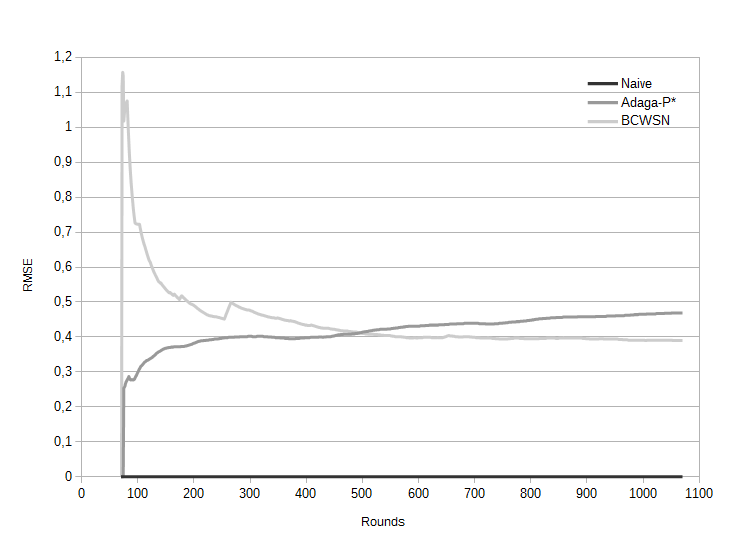
\includegraphics[scale=0.45]{BCWSN-RMSExRound-PB-Temp.png}
	 \vspace*{-.5cm}
    \caption{RMSE per round - Temperature}
    \label{fig:rmse}
\end{center}
\end{figure}

Figure \ref{fig:num-msg} depicts the number of transmitted messages
per round. In the Naive approach, the number of messages is steady, since in
each round all sensors send sensed data to the sink. It is important to observe
that, in average, BCWSN transmits $57.24\%$ less messages than Adaga-P* (see Table
\ref{tab:num-msg}). However, there are some peaks in BCWSN curve, which
represent periods in time when clusters are being restructured (splitting or
merging). Recall that BCWSN dynamically updates the cluster configuration. Such
a characteristic of the proposed approach is responsible for the high standard
deviation in Table \ref{tab:num-msg}.
%\vspace*{-.3cm}

\begin{figure}[!htb]
\begin{center}
	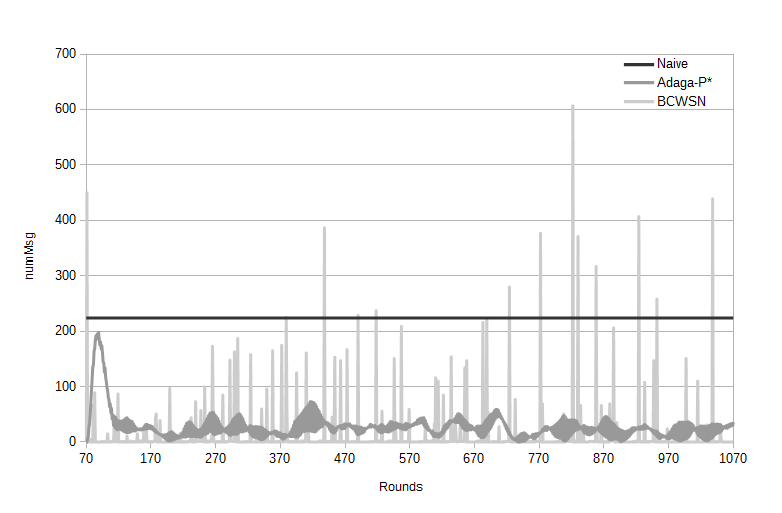
\includegraphics[scale=0.4]{BCWSN-NumMsgPerRoundxRound-PB.png}
	 \vspace*{-.6cm}
    \caption{Messages per round - Temperature}

    \label{fig:num-msg}
\end{center}
\end{figure}
%\vspace*{-.3cm}

In Figure \ref{fig:tot-num-msg}, the total number of messages sent by sensors in
BCWSN is much smaller compared to Adaga-P*, despite the wide variation in the
number of messages sent per round in the former (Figure \ref{fig:num-msg}).
%\vspace*{-.3cm}

Figure \ref{fig:num-clts} shows the variation in number of clusters from BCWSN 
that demonstrates how our proposal is able to adapt to changes in the sensed 
environment by changing the clusters to reflect such changes.
%\vspace*{-.3cm}

\begin{figure}[!htb]
\begin{center}
	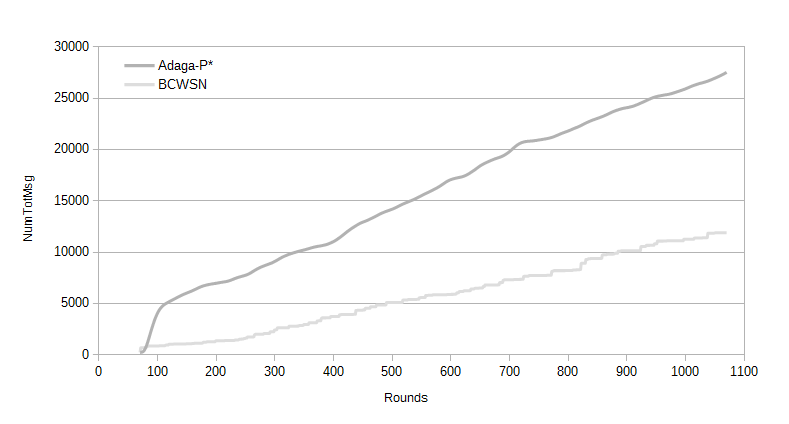
\includegraphics[scale=0.40]{BCWSN-TotNumMsgxRound-PB-2Appr.png}
	 \vspace*{-.6cm}
    \caption{Total number of messages - Temperature}
    \label{fig:tot-num-msg}
\end{center}
\end{figure}
\vspace*{-.3cm}

In Figure \ref{fig:rmse}, there is a peak for the BCWSN curve. The reason for
this is the fact that the first cluster formation is only an initialization step
for this approach. Thus the BCWSN accuracy is jeopardized at the beginning.
Nonetheless, the BCWSN approach is able to dynamically adjust the accuracy by
reducing the RMSE through the use of Fractal Clustering (FC) technique.
\vspace*{-.3cm}

\begin{figure}[!htb]
\begin{center}
	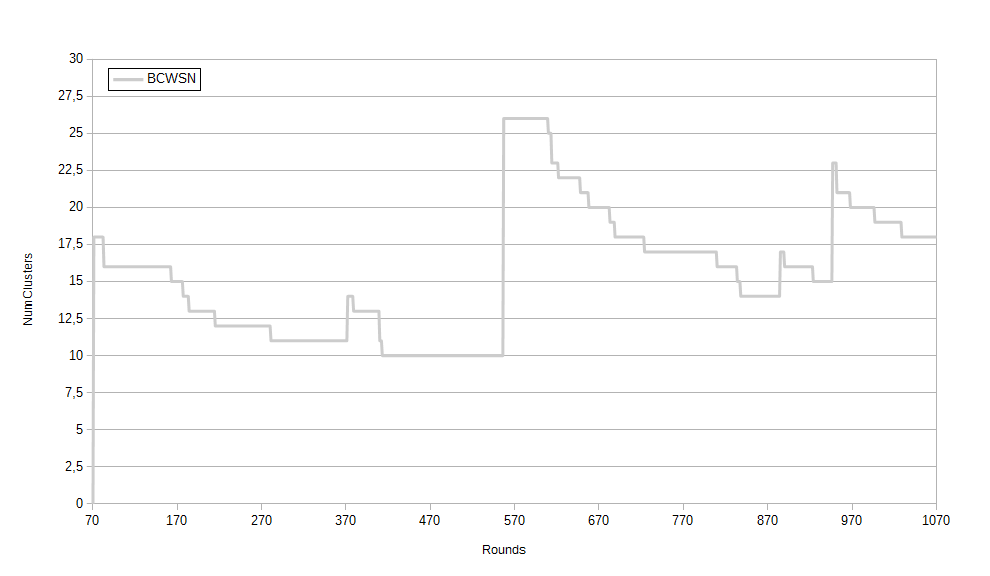
\includegraphics[scale=0.34]{BCWSN-NumClustersxRound-PB.png}
	 \vspace*{-.6cm}
    \caption{Number of clusters per round - Temperature}
    \label{fig:num-clts}
\end{center}
\end{figure}
%\vspace*{-.3cm}

Next, we present the test results for ``humidity', to show the efficiency of the
proposed proposal in a more general way.
%\vspace*{-.3cm}

\begin{figure}[!htb]
\begin{center}
	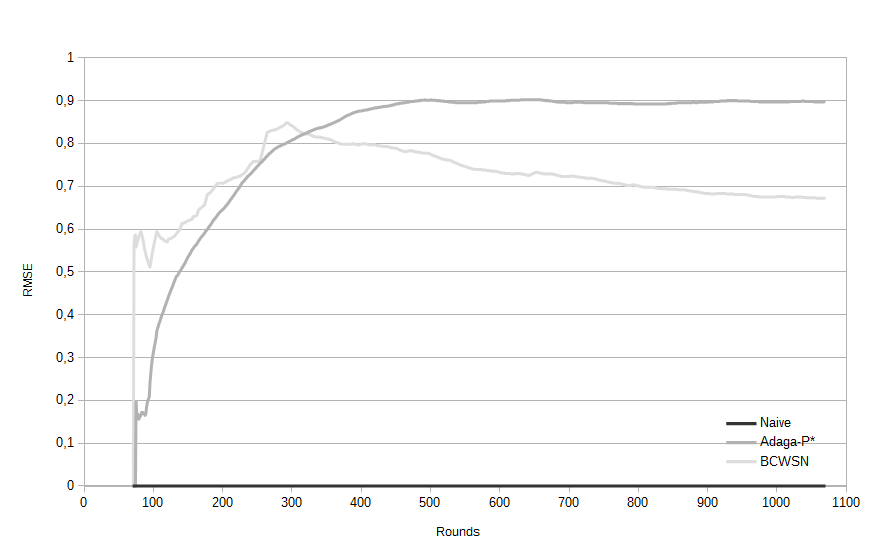
\includegraphics[scale=0.37]{BCWSN-RMSExRound-PB-Hum.png}
	 \vspace*{-.6cm}
    \caption{RMSE per round - Humidity}
    \label{fig:rmse-hum}
\end{center}
\end{figure}
\vspace*{-.3cm}

Figure \ref{fig:rmse-hum} shows that for 
humidity, BCWSN's RMSE  starts higher than Adaga-P*. however from a certain 
point in time (Round 320) on it drops lower than RMSE for Adaga-P*.
%\vspace*{-.3cm}

In Figure \ref{fig:tot-num-msg-hum}, one can see that the total number of messages 
in the case of BCWSN is also lower than the Adaga-P*. For the sake of clarity,
we did not included the Naive curve for total number of messages, because it is
too high w.r.t. the other two approaches.

\begin{figure}[!htb]
\begin{center}
	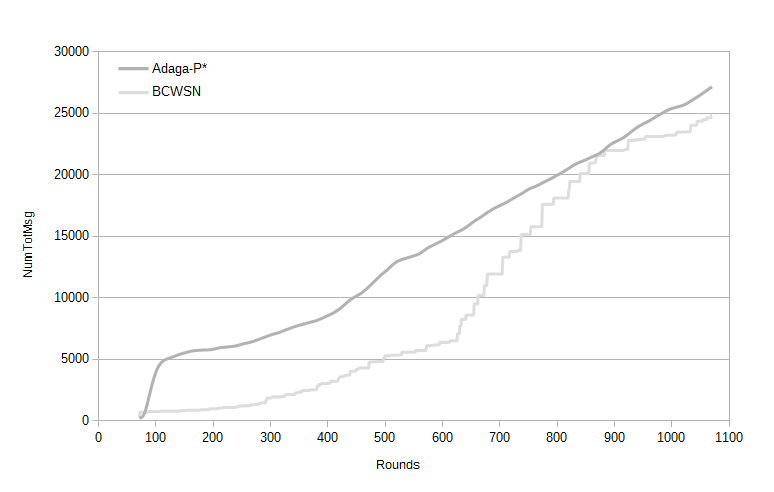
\includegraphics[scale=0.4]{BCWSN-TotNumMsgxRound-PB-2Appr-Hum.png}
	 \vspace*{-.6cm}
    \caption{Total number of messages - Humidity}
    \label{fig:tot-num-msg-hum}
\end{center}
\end{figure}
\vspace*{-.3cm}

\section{Conclusion}
\label{conclusion}

In this paper, we have described a new approach for clustering sensors in WSNs
based on the notion of Behavioral Correlation and Fractal Clustering.
Behavioral Correlation identifies sensors with similar data reading patterns,
among one or more (different) data type readings. Since environmental
conditions may vary in time, BCWSN dynamically adjusts the Behavioral
Correlation among the data collect by the sensor nodes.
\vspace*{-.3cm}

The results presented in Section \ref{results-and-discussion} show BCWSN may
significantly decrease energy consumption in WSNs, while assuring a low RMS
Error.
\vspace*{-.3cm}

%Currently, we are working on
%measuring distance between prediction models to assess the dissimilarity in
%sensed data behavior. Moreover, we are evaluating the use of traditional
%techniques of data mining, such as K-Means, to perform the initial grouping of
%sensors into clusters, overriding the use of similarity measures for such
%purpose.



\bibliographystyle{abbrv}
\bibliography{SAC2015rodrigues_brayner_maia}  
% SAC2015rodrigues_brayner_maia.bib is the name of the Bibliography in this case
% You must have a proper ".bib" file
%  and remember to run:
% latex bibtex latex latex
% to resolve all references

\end{document}